%************************************************
\chapter{Q-learning with CVaR}\label{ch:qlearning}
%************************************************

While value iteration is a useful algorithm, it only works when we have complete knowledge of the environment - including the probability transitions $p(x'|x,a)$. This is often not the case in practice and we have to rely on different methods, based on direct interaction with the environment. One such algorithm is the well-known Q-learning which we explore in this chapter.

We first remind the reader of Q-learning basics in \secref{qlearning} and introduce CVaR estimation in \secref{cvarestimation}. These concepts are combined together with CVaR value iteration and in \secref{qcvar} we propose the first CVaR Q-learning algorithm. We treat the optimal policy separately in \secref{qpolicy}.

The algorithm is then experimentally verified on suitable environments in \secref{qexperiments}.

%***********************************************************************************************************************************************************
%***********************************************************************************************************************************************************
%***********************************************************************************************************************************************************
\subsection{Q-learning}\label{sec:qlearning}

Q-learning (\citet{watkins1992q}) is an important off-policy temporal difference control algorithm, that works by repeatedly updating the $Q$ value estimate according to the sampled rewards and states using a moving exponential average.
\begin{equation}
\begin{split}
&Q_{t+1}(x, a) = (1-\beta)Q_{t}(x, a) + \beta\bsquare{r + \gamma \max_{a'} Q_t(x', a')}\\
&x' \sim p(\cdot|x, a)
\end{split}
\end{equation}
Here $Q$ is an estimate of the optimal action-value function \eqnref{q} and $\beta$ is the learning rate. The expression $r + \gamma \max_{a'} Q_t(x', a')$ is called a \textit{target} and is sometimes denoted as $\cT Q$. The idea of the algorithm is to bring the value function closer to the target, which is more 'informed' than the original value since it has information about the reward and next state, which came directly from the sampled transition.

The order of the visited states is unimportant, as long as all reachable states are updated infinitely often and the learning rate meets a standard condition used in stochastic approximation.
\begin{equation}\label{eqn:beta}
\sum_{t=0}^\infty \beta_t = \infty  \quad \sum_{t=0}^\infty \beta_t^2 < \infty\\
\end{equation}
See \citet{jaakkola1994convergence} for details.

While the algorithm would converge if we were using a completely random policy, in practice we often try to speed up the convergence by using a smarter, yet still random policy. See \algref{qlearning} for a full practical procedure.


\begin{algorithm}
\caption{Q-learning}
\begin{algorithmic}\label{alg:qlearning}
    \STATE Initialize $Q(x, a)$ for all $x \in \cX, a \in \cA$ arbitrarily, and $Q(x_\text{terminal}, \cdot) = 0$
    
	\FOR{each episode}
		
	\STATE $x = x_0$
	
	\WHILE{$x$ is not terminal}
	\STATE Choose $a$ using a policy derived from $Q$ (e.g. $\varepsilon$-greedy)
	\STATE Take action $a$, observe $r, x'$
	\STATE $Q(x, a) = (1-\beta)Q(x, a) + \beta\bsquare{r + \gamma \max_{a'} Q(x', a')}$
	\STATE $x = x'$	
	\ENDWHILE
	
	\ENDFOR
\end{algorithmic}
\end{algorithm}


\subsection{CVaR estimation}\label{sec:cvarestimation}

Before formulating a CVaR version of Q-learning, we must first talk about simply \emph{estimating} CVaR, as it is not as straightforward as the estimation of expected value.

Let us remind ourselves of the primal definition of CVaR \eqnref{cvarprimal}:
\begin{equation*}
\cvar_\alpha(Z)=
\max_s\left\lbrace \dfrac{1}{\alpha}\expect
\left[ (Z-s)^-\right] + s  \right\rbrace 
\end{equation*}
If we knew the exact $s^*=\var_\alpha$, we could estimate the CVaR as a simple expectation of the $\dfrac{1}{\alpha}(Z-s^*)^-+s^*$ function. As we do not know this value in advance, a common approach is to first approximate $\var_\alpha$ from data, then use this estimate to compute it's $\cvar_\alpha$. This is usually done with a full data vector, requiring the whole data history to be saved in memory.

When dealing with reinforcement learning, we would like to store our current estimate as a scalar instead. This requires finding a recursive expression whose expectation is the CVaR value. Fortunately, similar methods have been thoroughly investigated in the stochastic approximation literature by \citet{robbins1951stochastic}.

The RM theorem has also been applied directly to CVaR estimation by \citet{bardou2009recursive}, who used it to formulate a recursive importance sampling procedure useful for estimating CVaR of long-tailed distributions.

First let us describe the method for a one step estimation, meaning we sample values (or rewards in our case) $r$ from some distribution and our goal is to estimate CVaR at a given confidence level $\alpha$. The procedure requires us to maintain two separate estimates $V$ and $C$, being our VaR and CVaR estimates respectively.
\begin{align}
V_{t+1} &= V_{t} + \beta \bsquare{1-\dfrac{1}{\alpha}\indicator_{(V_t \ge r)}}\label{eqn:varestimate}\\
C_{t+1} &= (1-\beta)C_t + \beta \bsquare{V_t + \dfrac{1}{\alpha}(r-V_t)^-}\label{eqn:cvarestimate}
\end{align}

An observant reader may recognize a standard equation for quantile estimation in equation \eqnref{varestimate} (see e.g. \citet{koenker2001quantile} for more information on quantile estimation/regression) and equation \eqnref{cvarestimate} is also quite intuitive, representing the moving exponential average of the primal CVaR definition \eqnref{cvarprimal}. The estimations are proven to converge, given the usual requirements on the learning rate \eqnref{beta} \citep{bardou2009recursive}.

%***********************************************************************************************************************************************************
%***********************************************************************************************************************************************************
%***********************************************************************************************************************************************************

\section{CVaR Q-learning}\label{sec:qcvar}

We now extend the previously established CVaR value iteration and combine it with the recursive CVaR estimation techniques to formulate a new algorithm we call CVaR Q-learning.
\subsection{Temporal Difference update}
We first define two separate values for each state, action and atom $V, C: \cX\times\cA\times\cY\to\real$ where $C(x, a, y)$ represents $\cvar_y(Z(x, a))$ of the distribution, similar to the definition \eqnref{cdef}. $V(x, a, y)$ represents the one-step $\var_y$ estimate, or the estimate of the $y-$quantile of a distribution recovered from $\cvar_y$ by Lemma \ref{thm:varcvarconnection}.

A key to any temporal difference algorithm is it's update rule. The CVaR TD update rule extends the improved VI procedure and we present the full rule in \algref{cvartd}. 

Let us now go through the algorithm and compare the two versions. We first construct a new CVaR (line \ref{alg:cvartd:1}), representing CVaR of $Z(x')$, by greedily selecting actions that yield the highest CVaR for each atom. This step is somewhat skipped in the VI procedure since we are not working with action-value functions. These values are then transformed to their underlying distributions (line \ref{alg:cvartd:2}) and used to generate samples from this distribution. Since we know the distribution estimates exactly, we do not have to actually sample - instead we use the quantile values proportionally to their probabilities and apply the respective VaR and CVaR update rules (lines \ref{alg:cvartd:4}, \ref{alg:cvartd:5}).

Note that if the atoms aren't uniform, we perform basic importance sampling in the expectation terms, weighting each 'sample' according to it's probability. 

%\begin{align*}
%\expect_j\bsquare{1 - \dfrac{1}{y_i}\indicator_{(V(x, a, y_i) \ge r+\gamma d_j)}} &= \sum_j (y_j - y_{j-1})\bsquare{1 - \dfrac{1}{y_i}\indicator_{(V(x, a, y_i) \ge r+\gamma d_j)}}\\
%\expect_j\bsquare{V(x, a, y_i) + \dfrac{1}{y_i}\bround{r+\gamma d_j - V(x, a, y_i)}^-} &= kok
%\end{align*}

\begin{algorithm}
\caption{CVaR TD update}
\begin{algorithmic}[1]\label{alg:cvartd}

    \STATE \textbf{input:} $x, a, x', r$
    
    \FOR{each $y_i$ }
	\STATE $C(x', y_i) = \max_{a'} C(x', a', y_i)$ \label{alg:cvartd:1}
	\ENDFOR
	
	\STATE $\mathbf{d}= \text{extractDistribution}\bround{C(x', \mathbf{y})}$ \label{alg:cvartd:2}

	\FOR{each $y_i$}
	\STATE $V(x, a, y_i) = V(x, a, y_i) + \beta \expect_j\bsquare{1 - \frac{1}{y_i}\indicator_{(V(x, a, y_i) \ge r+\gamma d_j)}}$  \label{alg:cvartd:4}
	\STATE $C(x, a, y_i) = (1-\beta)C(x, a, y_i) + \beta\expect_j\bsquare{V(x, a, y_i) + \frac{1}{y_i}\bround{r+\gamma d_j - V(x, a, y_i)}^-}$\label{alg:cvartd:5}
	\ENDFOR
\end{algorithmic}
\end{algorithm}

\subsection{Note on convergence}
We do not prove the convergence of the CVaR Q-learning algorithm in this thesis as it would require significant work regarding convergence of the recursive CVaR estimation procedure. The update rules (\ref{eqn:varestimate}, \ref{eqn:cvarestimate})  have been only shown to converge if the underlying distributions are continuous \citep{bardou2009recursive}, which is not the case in our setting.


In the last section of this chapter, we show at least empirical convergence of the CVaR Q-learning algorithm.

%***********************************************************************************************************************************************************
%***********************************************************************************************************************************************************
%***********************************************************************************************************************************************************


\section{Optimal Policy}\label{sec:qpolicy}

Recall that in CVaR Value Iteration we can extract the optimal policy by recursively setting $y_{t+1}=y_t \xi^*_{x_{t+1}}$. This process is not straightforwardly extendable to our sample-based version of CVaR VI, since we would have to have acces to all possible transition states and probabilities in order to compute $\xi^*$.

Instead, we turn to the primal formulation of CVaR in what we call VaR-based policy improvement algorithm.

\subsection{VaR-based Policy Improvement}

We first introduce the VaR-based policy improvement in the context of distributional RL and extend it to CVaR Q-learning in the next section.

Let us now assume that we have succesfully converged with distributional value iteration and therefore have available the return distributions of some stacionary policy for each state and action. Our next goal is to find a policy improvement algorithm that will monotonically increase the $\acvara$ criterion for selected $\alpha$.

Recall the primal definition of CVaR \eqnref{cvarprimal}
\begin{equation*}
\text{CVaR}_\alpha(Z)=
\max_s\left\lbrace \dfrac{1}{\alpha}\expect
\left[ (Z-s)^-\right] + s  \right\rbrace 
\end{equation*}
Our goal \eqnref{problem} can then be rewritten as
\begin{equation*}
\max_\pi CVaR_\alpha^\pi(Z) = \max_\pi \max_s \dfrac{1}{\alpha}\mathbb{E}
\left[ (Z^\pi-s)^-\right] + s
\end{equation*}
As mentioned earlier, the primal solution is equivalent to $\var_\alpha(Z)$
\begin{equation*}
\text{CVaR}_\alpha(Z)=
\max_s\left\lbrace \dfrac{1}{\alpha}\mathbb{E}
\left[ (Z-s)^-\right] + s  \right\rbrace =\dfrac{1}{\alpha}\mathbb{E}
\left[ (Z - \text{VaR}_\alpha(Z))^-\right] + \text{VaR}_\alpha(Z) 
\end{equation*}

The main idea of VaR-based policy improvement is the following: If we knew the value $s^*$ in advance, we could simplify the problem to maximize only
\begin{equation}\label{eqn:varbasedgoal}
\max_\pi CVaR_\alpha(Z^\pi) = \max_\pi \dfrac{1}{\alpha}\mathbb{E}
\left[ (Z^\pi-s^*)^-\right] + s^*
\end{equation}
Given that we have access to the return distributions, we can improve the policy by simply choosing an action that maximizes $\cvar_\alpha$ in the first state $a_0 = \text{arg}\max_\pi\text{CVaR}_\alpha(Z^\pi(x_0))$, setting $s^* = VaR_\alpha(Z(x_0))$ and focus on maximization of the simpler criterion.

This can be seen as coordinate ascent; in the first phase (when we compute CVaR) we maximize w.r.t. $s$ while keeping $\pi$ fixed; in the second phase we fix $s$ and maximize w.r.t. $\pi$.

The extension to MDPs consists of recursively updating the $s$ we maximize by setting $s = \dfrac{s - r_t}{\gamma}$. See \algref{varbasedpi} for the full procedure which we justify in the following theorem.

\begin{algorithm}
\caption{VaR-based policy improvement}
\label{alg:varbasedpi}
\begin{algorithmic}
    \STATE $a = \text{arg}\max_a CVaR_\alpha(Z(x_0, a))$
    \STATE $s = VaR_\alpha(Z(x_0, a))$
    \STATE $x_t, r_t = \text{envTransition}(x_0, a)$
    \WHILE{$x_t$ is not terminal}
    	\STATE $s = \dfrac{s-r_t}{\gamma}$
    	\STATE $a = \text{arg}\max_a \mathbb{E}\left[(Z(x_t, a)-s)^- \right]$
    	\STATE $x_t, r_t = \text{envTransition}(x_t, a)$
   	\ENDWHILE
\end{algorithmic}
\end{algorithm}

\begin{theorem}
Let $\pi$ be a stationary policy, $\alpha \in (0, 1]$. 
By following policy $\pi'$ from algorithm \ref{alg:varbasedpi}, we improve $CVaR_\alpha(Z)$ in expectation:
$$CVaR_\alpha(Z^\pi) \le CVaR_\alpha(Z^{\pi'})$$
%
%Let policy $\pi'$ constructed the following way: Set $\pi'(x_0) = \text{arg}\max_\pi\cvar_\alpha(Z^\pi(x_0))$ and $s = \var_\alpha(Z^\pi(x_0, \pi'(x_0)))$. Each following step set $s = $
%

\end{theorem}

\begin{proof}

Let $s^*$ be a solution to \eqnref{cvarprimal}. Then by optimizing $\max_\pi \dfrac{1}{\alpha}\mathbb{E}
\left[ (Z^\pi-s^*)^-\right]$, we monotonely improve the optimization criterion \eqnref{problem}.
\begin{align*}
CVaR_\alpha(Z^{\pi}) &= \max_{s}\dfrac{1}{\alpha}\mathbb{E}\left[ (Z^{\pi'}-s)^-\right] + s \\
&\le \max_{\pi'}\dfrac{1}{\alpha}\mathbb{E} \left[ (Z^{\pi'}-s^*)^-\right] + s^*\\
 &\le \max_{s'}\dfrac{1}{\alpha}\mathbb{E}\left[ (Z^{\pi'}-s')^-\right] + s' = CVaR_\alpha(Z^{\pi'})
\end{align*}

%The last equation holds if $Z\sim p_i$ is a probability mixture for any function $H$.
%Here $Z_{t+1} \sim P(x_{t+1}\given x_t, a)$ represents the random variable mixture when we do not yet know which transition was sampled.
%We further simplified the notation by assigning indices $i$ to each of the possible $x_{t+1}$.
We can rewrite our subgoal as
\begin{equation}
\begin{split}
\mathbb{E}\left[(Z_t-s)^-\right] &= \mathbb{E}\left[(Z_t-s)\mathbb{1}(Z_t\le s)\right] = \mathbb{E}\left[(R_t + \gamma Z_{t+1}-s)\mathbb{1}(Z_{t+1}\le \dfrac{s - R_t}{\gamma})\right]\\
&= \sum_{x_{t+1}, r_t} P(x_{t+1}, r_t \given x_t, a)\mathbb{E}\left[(r_t + \gamma Z(x_{t+1})-s)\mathbb{1}(Z(x_{t+1})\le \dfrac{s - r_t}{\gamma})\right]\\
&= \sum_{x_{t+1}, r_t} P(x_{t+1}, r_t \given x_t, a)\mathbb{E}\left[\gamma\left(Z(x_{t+1})-\dfrac{s-r_t}{\gamma}\right)\mathbb{1}(Z(x_{t+1})\le \dfrac{s - r_t}{\gamma})\right]\\
&= \gamma\sum_{x_{t+1}, r_t} P(x_{t+1}, r_t \given x_t, a)\mathbb{E}\left[\left(Z(x_{t+1})-\dfrac{s-r_t}{\gamma}\right)\mathbb{1}(Z(x_{t+1})\le \dfrac{s - r_t}{\gamma})\right]\\
&= \gamma\sum_{x_{t+1}, r_t} P(x_{t+1}, r_t \given x_t, a)\mathbb{E}\left[\left(Z(x_{t+1}) - \dfrac{s - r_t}{\gamma}\right)^-\right]
\end{split}
\end{equation}
where we used the definition of return $Z_t = R_t + \gamma Z_{t+1}$ and the fact that probability mixture expectations can be computed as $\mathbb{E}[f(Z)] = \sum_i p_i \mathbb{E}[f(Z_i)]$ for any function $f$.

Now let's say we sampled reward $\hat{r}_t$ and state $\hat{x}_{t+1}$, we are still trying to find a policy $\pi^*$ that maximizes 
\begin{equation}\label{eqn:sampled x_t+1}
\begin{split}
\pi^* &=\text{arg}\max_\pi \mathbb{E}\left[(Z_t-s)^-\right | \hat{x}_{t+1}, \hat{r}]\\
&= \text{arg}\max_\pi \mathbb{E}\left[\left(Z(\hat{x}_{t+1}) - \dfrac{s - \hat{r}_t}{\gamma}\right)^-\right]
\end{split}
\end{equation}

Where, by the linearity of the expected value, we ignored the unsampled states (since these are not a function of $\hat{x}_{t+1}$) and the multiplicative constant $\gamma$ that will not affect the maximum argument.

At the starting state, we set $s=s^*$. At each following state we select an action according to equation \eqnref{sampled x_t+1}. By induction we maximize the criterion \eqnref{varbasedgoal} in each step.
\end{proof}

Note that while the resulting policy is nonstationary, we do not need an extended state-space to follow this policy. It is only necessary to remember our previous value of $s$.

\subsection{CVaR Q-learning extension}
We would now like to use the policy improvement algorithm in order to extract the optimal policy from CVaR Q-learning. Unfortunately we cannot straightforwardly maximize $\mathbb{E}\left[(Z_t-s^*)^-\right]$ since the Value-at-Risk estimates $V$ we have do not reflect the actual VaR of the return. Instead they represent the one-step VaR of a distribution extracted from the optimal CVaR.

To side-step this issue, we bring the VaR-based improvement closer to CVaR VI and use it only in a one-step context. In each step, we compute the next $y$ as $F_{Z(x)}(\dfrac{s-r}{\gamma})$, which we extract from our VaR estimate $V$. Since we don't have access to the exact VaR for each $y \in [0,1]$ due to discretization, we use linear interpolaton as a heuristic. See \algref{varxibasedpolicy} for the full procedure.
\begin{algorithm}
\caption{CVaR Q-learning policy}\label{alg:varxibasedpolicy}
\begin{algorithmic}
    \STATE \textbf{input:} $\alpha$, converged $V(x, a, y), C(x, a, y)$
    		
	\STATE $x = x_0$
	\STATE $y = \alpha$
	\STATE $s = V(x, a, y)$
	\WHILE{$x$ is not terminal}
	\STATE $a = \argmax_a C(x, a, y)$
	\STATE Take action $a$, observe $r, x'$
	\STATE $y = F_{Z(x')}(\dfrac{s-r}{\gamma})$
	\STATE $s = V(x, a, y)$
	\STATE $x = x'$
	\ENDWHILE
\end{algorithmic}
\end{algorithm}

\todo{end section, full cvar q?}

%\begin{algorithm}
%\caption{Full CVaR Q-learning}
%\begin{algorithmic}
%    \STATE Initialize $V(x, a, y), C(x, a, y)$ for all $x\in\cX, a\in\cA, y\in\cY$ arbitrarily, and $C(x_\text{terminal}, \cdot, \cdot) = 0$
%    
%	\FOR{each episode}
%		
%	\STATE $x = x_0$
%	\STATE $y = \alpha$
%	\STATE $s = V(x, a, y)$
%	\WHILE{$x$ is not terminal}
%	\STATE Choose $a$ using a policy derived from $C, y$ (e.g. $\varepsilon$-greedy)
%	\STATE Take action $a$, observe $r, x'$
%	\STATE Update current estimates $V(x, a, y_i), C(x, a, y_i)$ (\algref{cvartd})
%	\STATE $y = F_{Z(x')}(\dfrac{s-r}{\gamma})$
%	\STATE $s = V(x, a, y)$
%	\STATE $x = x'$
%	\ENDWHILE
%	
%	\ENDFOR
%\end{algorithmic}
%\end{algorithm}


%*****************************************
%*****************************************
%*****************************************


\section{Experiments}\label{sec:qexperiments}
We use the same gridworld from \secref{vi:experiments} with $\delta=0.1$. Since the positive reward is very sparse, we chose to run CVaR Q-learning on a smaller environment of size $10\times15$. We trained the agent for 10,000 sampled episodes with $\gamma=0.99$, learning rate $\beta=0.4$ that dropped each 10 episodes by a factor of 0.995. The used policy was $\varepsilon-$greedy and maximized expected value ($\alpha=1$) with $\varepsilon=0.5$.

See \figref{qgrid} for learned policies with $N=50$ linearly-spaced atoms and \figref{qhist} for comparisons 

\begin{figure}[h]
\center
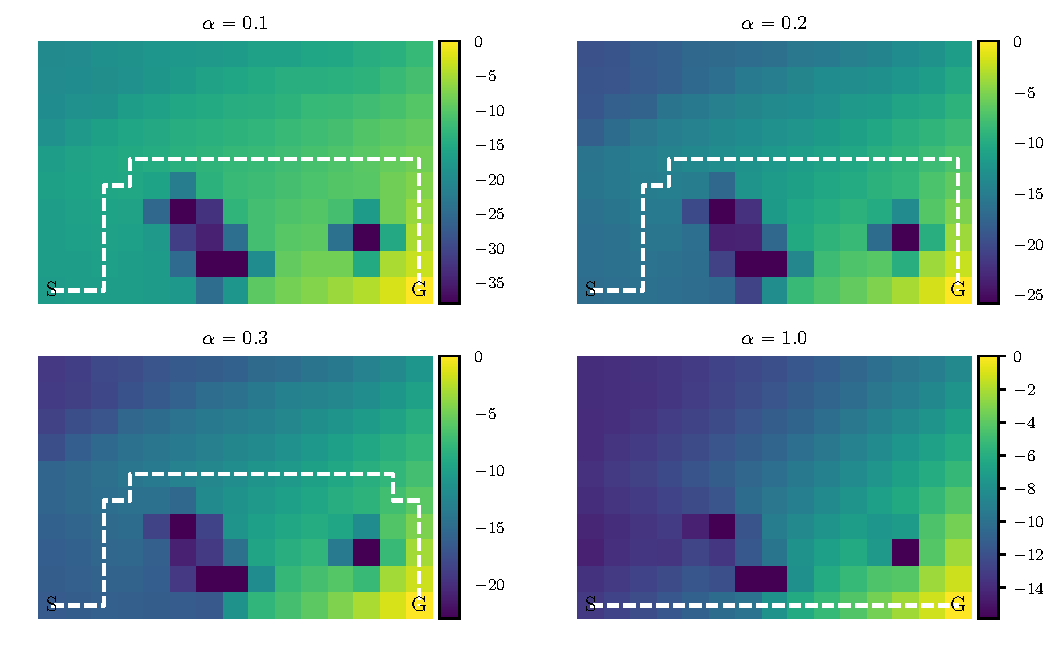
\includegraphics[width=\linewidth]{gfx/q_optimal_paths.pdf}
\caption{Grid-world Q-learning simulations. The optimal deterministic paths are shown together with CVaR estimates for given $\alpha$s.}
\label{fig:qgrid}
\end{figure}


\begin{figure}[h]
\center
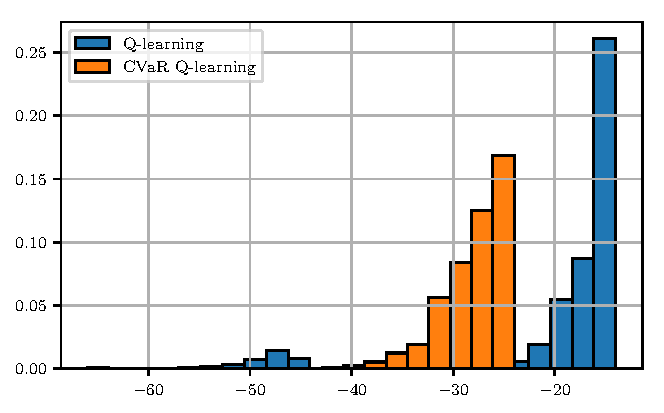
\includegraphics[width=0.6\linewidth]{gfx/sample_hist.pdf}
\caption{Sample histograms for policies generated by Q-learning and CVaR Q-learning with $\alpha=0.1$.}
\label{fig:qhist}
\end{figure}

We experimented with several discretization settings and didn't find many differences between log- and linearly-spaced atoms. One must however keep in mind that learning $\var$ and $\cvar$ for very low $\alpha$ values requires large number of samples and we found that extremely small atom values converged slowly.
\\
\\
\textit{Note on convexity:} Unlike CVaR Value Iteration, where we maintain convexity of the $y\cvar_y$ function with each update (given we started with convex estimates), we can break the convexity in each update for any atom. We experience this in practice as well as can be gauged from \figref{nonconvex}. Fortnately this fact does not break the update rule, since the targets we use to update $C$ as well as $V$ do not have to be in order.


\begin{figure}[h]
\center
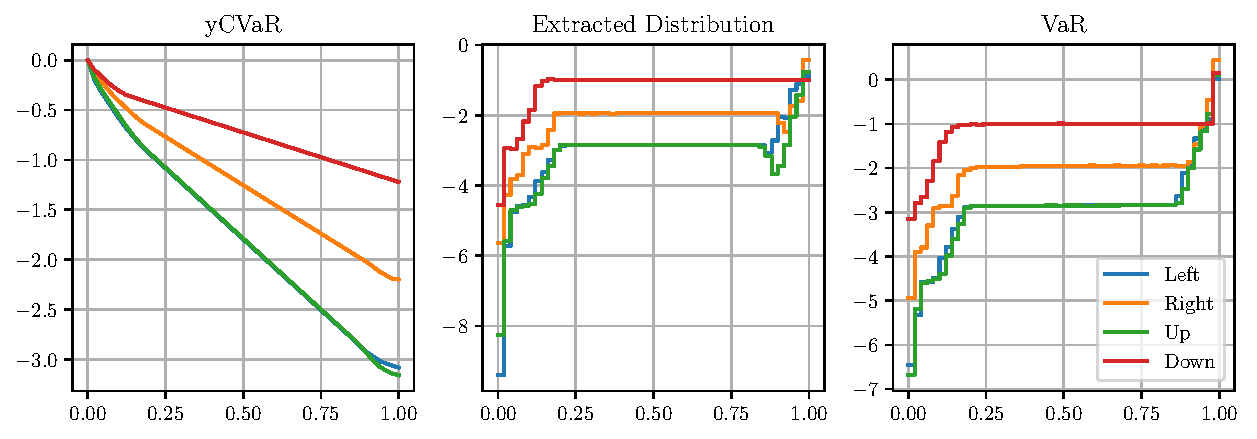
\includegraphics[width=\linewidth]{gfx/nonconvex.pdf}
\caption{Learned $C, V$ estimates after 10000 episodes. Notice the nonconvexities visible from the extracted distribution plot.}
\label{fig:nonconvex}
\end{figure}

\section{Summary}



%*****************************************
%*****************************************
%*****************************************
%*****************************************
%*****************************************
